% Slides from Lecture-10 lines 31--82 (main already inputs sections/cover).
\begin{frame}[plain]
  \centering
  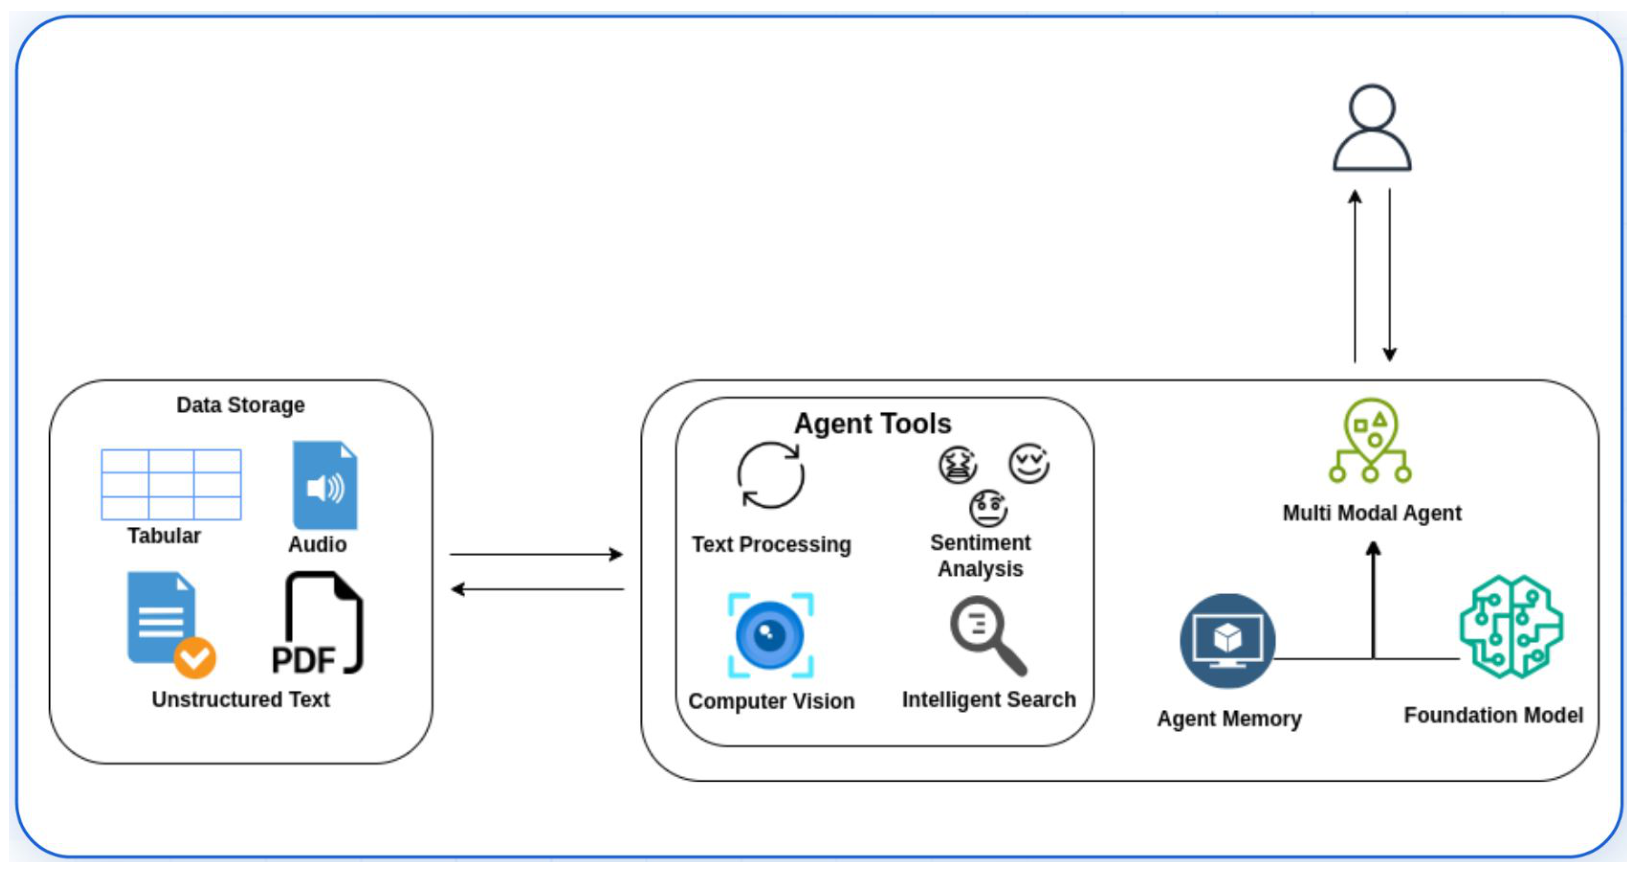
\includegraphics[width=0.8\paperwidth,height=0.8\paperheight,keepaspectratio]{assets/Lecture-10_Multimodal_NLP_Agentic_AI/slide_002.png}
\end{frame}

\begin{frame}{Table of Contents}
  \begin{enumerate}
    \item Motivation
    \item Learning Outcomes
    \item Vision-Language Models
      \begin{enumerate}
        \item CLIP: Contrastive Language-Image Pretraining
        \item VisualBERT
        \item FLAVA: Fusion of Language And Vision Architecture
      \end{enumerate}
    \item Multimodal Architectures
      \begin{enumerate}
        \item Categories of Multimodal Architectures
        \item Challenges in Multimodal Integration
      \end{enumerate}
    \item Agentic AI
      \begin{enumerate}
        \item What is Agentic AI?
        \item Reactive vs. Proactive Agents
      \end{enumerate}
  \end{enumerate}
\end{frame}

\begin{frame}{Table of Contents (contd.)}
  \begin{enumerate}
    \setcounter{enumi}{2}
    \item \textcolor{red}{Agent Loop}
    \setcounter{enumi}{5}
    \item \textcolor{red}{Open-Source Agentic Frameworks}
      \begin{enumerate}
        \item Auto-GPT
        \item BabyAGI
        \item Other Notable Frameworks
      \end{enumerate}
    \item Continual Learning in Agents
      \begin{enumerate}
        \item Why Continual Learning?
        \item Challenges in Continual Learning
      \end{enumerate}
    \item Safety, Ethics\hspace{0.2em} Control
      \begin{enumerate}
        \item Safety in Agentic Systems
        \item Ethics and Control
      \end{enumerate}
    \item Future Directions
  \end{enumerate}
\end{frame}
